\documentclass[portrait,a0paper,fontscale=0.29]{baposter}

\usepackage{fourier}
\usepackage[T1]{fontenc}
\usepackage[utf8]{inputenc}
\usepackage{graphicx}
\usepackage{amsmath} % typesetting math
\usepackage{amssymb}
\usepackage{upgreek} %proper greek letters
\usepackage{booktabs} % nice tables
%\usepackage{amsfonts,amssymb,amscd}
\newcommand{\unit}[1]{\ensuremath{\, \mathrm{#1}}}
\usepackage[none]{hyphenat}%no hyphenation

%%%%%%%%%%%%%%%%%%%%%%%%%%%%%%%%%%%%%%%%%%%%%%%%%%%%%%%%%%%%%%%%%%%%%%%%%%%%%%%%
% Multicol Settings
%%%%%%%%%%%%%%%%%%%%%%%%%%%%%%%%%%%%%%%%%%%%%%%%%%%%%%%%%%%%%%%%%%%%%%%%%%%%%%%%
\setlength{\columnsep}{0.7em}
\setlength{\columnseprule}{0mm}

%%%%%%%%%%%%%%%%%%%%%%%%%%%%%%%%%%%%%%%%%%%%%%%%%%%%%%%%%%%%%%%%%%%%%%%%%%%%%%%%
% Save space in lists. Use this after the opening of the list
%%%%%%%%%%%%%%%%%%%%%%%%%%%%%%%%%%%%%%%%%%%%%%%%%%%%%%%%%%%%%%%%%%%%%%%%%%%%%%%%
\newcommand{\compresslist}{%
\setlength{\itemsep}{1pt}%
\setlength{\parskip}{0pt}%
\setlength{\parsep}{0pt}%
}
\xdefinecolor{framecolor}{HTML}{2B214A}
\xdefinecolor{accentcolor}{HTML}{9690A8}
\xdefinecolor{offwhitecolor}{HTML}{F7F6F8}

\begin{document}
%%%%%%%%%%%%%%%%%%%%%%%%%%%%%%%%%%%%%%%%%%%%%%%%%%%%%%%%%%%%%%%%%%%%%%%%%%%%%
%% Here starts the poster
%%---------------------------------------------------------------------------
%% Format it to your taste with the options
%%%%%%%%%%%%%%%%%%%%%%%%%%%%%%%%%%%%%%%%%%%%%%%%%%%%%%%%%%%%%%%%%%%%%%%%%%%%%
\begin{poster}{
 % Show grid to help with alignment
 grid=false,
 columns=3,
 % Column spacing
 colspacing=0.6em,
 % Color style
 headerColorOne=framecolor,
 headerFontColor=offwhitecolor,
 borderColor=framecolor,
 headershade=plain,
 % Format of textbox
 textborder=roundedsmall,
 % Format of text header
 headerborder=open,
 headerfont=\Large\textsc,
 headershape=smallrounded,
 headershade=plain,
 background=plain,
 bgColorOne=offwhitecolor,
 boxColorOne=offwhitecolor,
 headerheight=0.13\textheight}
 % Eye Catcher
 { \parbox[c]{0.11\textwidth}{
\includegraphics[width=0.11\textwidth]{logo/insa} \\
\includegraphics[width=0.11\textwidth]{logo/creatis} \\ 
\includegraphics[width=0.11\textwidth]{logo/ipnl}}
 }
 % Title
 {\Huge Performance of Prompt Gamma fall-off detection in clinical simulations}
 % Authors
 {
 \vspace{0.2cm}
 B.F.B. Huisman$^{1,2}$, É. Testa$^2$, D. Sarrut$^1$\\
 \begin{small}
 $^1$ CREATIS, Université de Lyon; CNRS UMR5220; INSERM U1044; INSA-Lyon;
\vspace{-0.2cm}
Université Lyon 1; Centre Léon Bérard, Lyon, France
 $^2$ IPNL, Université de Lyon; CNRS/IN2P3 UMR5822; Université Lyon 1 Lyon, France
 \end{small}\vspace{0.2cm}\\
 mail@brenthuisman.net
 }
 % University logo
 { \parbox[c]{0.11\textwidth}{
\includegraphics[width=0.11\textwidth]{logo/clb} \\       
\includegraphics[width=0.11\textwidth]{logo/labexprimes} \\ 
\includegraphics[width=0.11\textwidth]{logo/arclogo}}
 }
 
%%%%%%%%%%%%%%%%%%%%%%%%%%%%%%%%%%%%%%%%%%%%%
% Poster Text
%%%%%%%%%%%%%%%%%%%%%%%%%%%%%%%%%%%%%%%%%%%%%
\headerbox{1. Purpose}{name=objective,column=0,row=0,span=1}{

As the first Prompt Gammas (PG) cameras are deployed in clinical setting, we studied PG fall-off positions (FOP) estimation on a complete clinical simulations. The number of protons (spot weight) required for a consistent FOP estimate was investigated for two PG cameras, a multiparallel slit (MPS) and knife-edge slit (KES) design, for a single spot of a fully clinical Monte Carlo simulation of a patient treatment. \textbf{A new spot-grouping method is proposed that combines better measurement statistics with fall-off preservation.}
\\
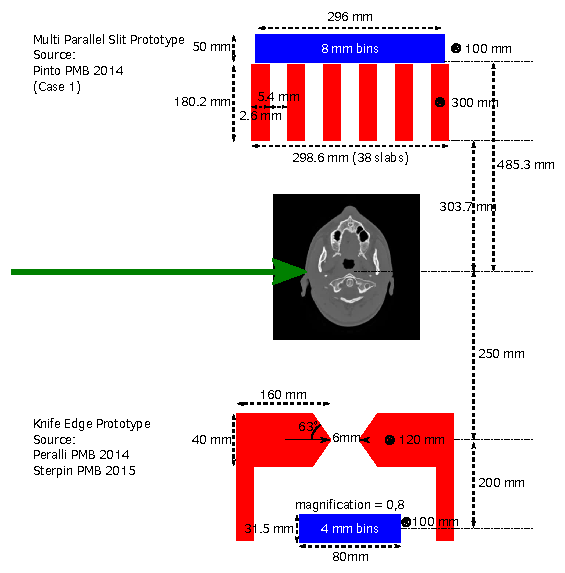
\includegraphics[width=0.99\textwidth]{pics/detectors}
}

\headerbox{2. Treatment plan analysis}{name=context,column=0,below=objective,span=1}{

By studying recent treatment plans from various proton clinics, we observe very few spots with weights over $10^8$ protons. The number of spots can vary over more than an order of magnitude per plan, and therefore spot intensities inversely vary over an order of magnitude as well. The negative correlation between the typical spot weight and plan robustness is an important observation, and presents a challenge: in robust plans where precision is required, and treatment verification seems most pertinent, PG cameras must be able to deal with lower spot weights than previously anticipated (less than <$10^7$ protons).

The remainder of the study investigates the number of primaries required for a usable PG signal. The spots in second field of the following treatment plan are considered:
\\
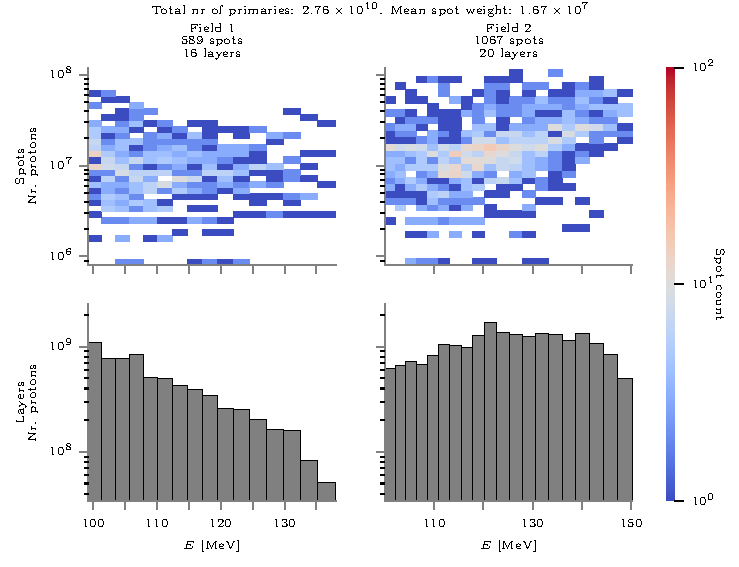
\includegraphics[width=0.99\textwidth]{pics/plannonorm-plot}
}

\headerbox{Acknowledgments}{name=ack,column=0,below=context,span=1}{
This work was partly supported by SIRIC LYric Grant INCa-DGOS-4664, LABEX PRIMES (ANR-11-LABX-0063 / ANR-11-IDEX-0007) and Fondation ARC.
}

\headerbox{3. Methods Modulated Spot}{name=conclu,column=1,span=1}{

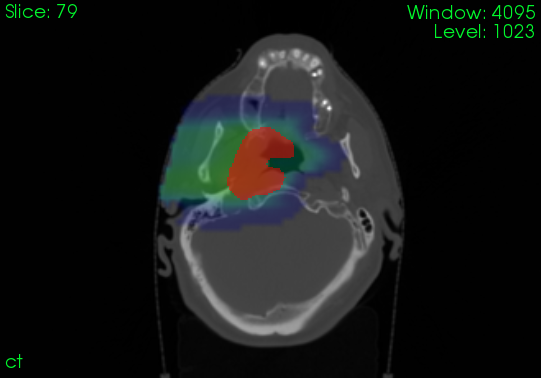
\includegraphics[width=0.99\textwidth]{pics/ourpatient}
\\
We considered a clinical head and neck case for which both a CT and re-planning (RP)CT were available. The patient had suffered from significant weight loss, which should translate to an expected shift in the dose and PG profiles. A treatment plan was created for the CT image (see Section 2), and it was irradiated on both CT and RPCT in silico using the vpgTLE mechanism available in Gate/Geant4 (Huisman et al.~2016). During the irradiation, two PG cameras implemented as published (Pinto et al.~2014, Peralli et al.~2014), recorded the PG profiles, spot by spot. We study shifted distributions as function of the spot weights, for each camera, from $10^6-10^9$ primaries. A FOP estimation was applied on 50 CT and 50 RPCT realizations to obtain FOP distributions for both images. Then, 2500 possible measured FOP shift were compiled by comparing each CT and RPCT FOP.% The standard deviation of this FOP shift distribution is a measure for the precision of a particular PG measurement: to what does a particular measured spot shift represent the actual shift?

}

\headerbox{4. Result Modulated Spot}{name=noise,column=1,below=conclu,span=1}{

FOP shifts detected by the MPS camera, as function of primary protons, for a spot A are shown below. The results at the prescribed spot weight ($4.7\cdot10^7$) or less result in standard deviations too large to warrant further investigation, which is why they are omitted from the rest of this study.

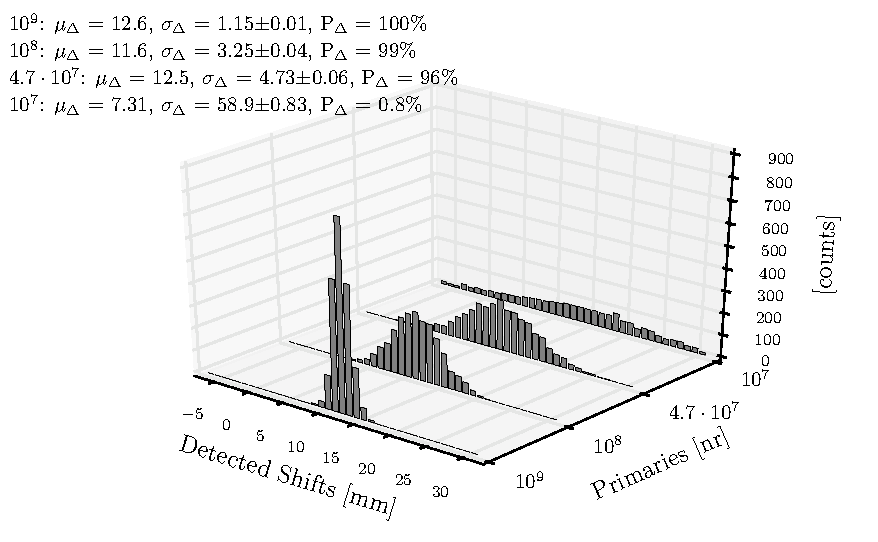
\includegraphics[width=0.99\textwidth]{{{pics/spot61-ipnl-auger-tof-1.root-FOP-shift}}}
Tabulated measured (mean) FOP shifts ($\upmu_\Delta\pm\upsigma$), for three selected spots, for both cameras, for both $10^9$ and $10^9$ primaries are shown below. They may be compared to the FOPs obtained for the Dose profile, PG emission profile and a point spread function applied to the PG emission, which models the PG transport from emission to detection. All numbers are in units of millimeters.\\

{\small
\begin{tabular}{llll}
	 & Spot A & Spot B & Spot C \\
	\midrule
	Dose & 2.77 & 4.08 & 12.4\\
	PG emission & 2.32 & 3.34 & 13.9\\
	PG + PSF & 2.61 & 2.91 & 11.9\\
	$\upmu_\Delta$ MPS @ $10^9$      & 2.68$\pm$0.77 & 3.23$\pm$0.77 & 12.6$\pm$1.15 \\
	$\upmu_\Delta$ KES @ $10^9$      & 2.56$\pm$1.93 & 3.27$\pm$2.24 & 9.79$\pm$2.25 \\
	$\upmu_\Delta$ MPS @ $10^8$      & 2.83$\pm$1.90 & 3.12$\pm$2.14 & 11.6$\pm$3.25 \\
	$\upmu_\Delta$ KES @ $10^8$      & 3.90$\pm$9.71 & 2.90$\pm$13.3 & 7.01$\pm$16.2 \\
\end{tabular}
}
}

\headerbox{5. Methods Spot Grouping}{name=mettwee,column=2,span=1}{

A natural way to improve statistics is to integrate PG profiles over multiple spots. We investigate if and how spot-grouping methods improve FOP estimation. We took all spots in the iso-energy layer of spot A and compared the results with an iso-depth grouping for spot A. Iso-depth grouping revolves around pre-computing the FOP on the dose profiles beforehand, which is clinically implementable in a TPS. In the plot below, the number of spots are binned according to their dose FOPs (red) and multiplied with their respective spot weights plotted in green. For comparison, the dose profile (cumulative over all spots) is plotted in blue (not to scale).

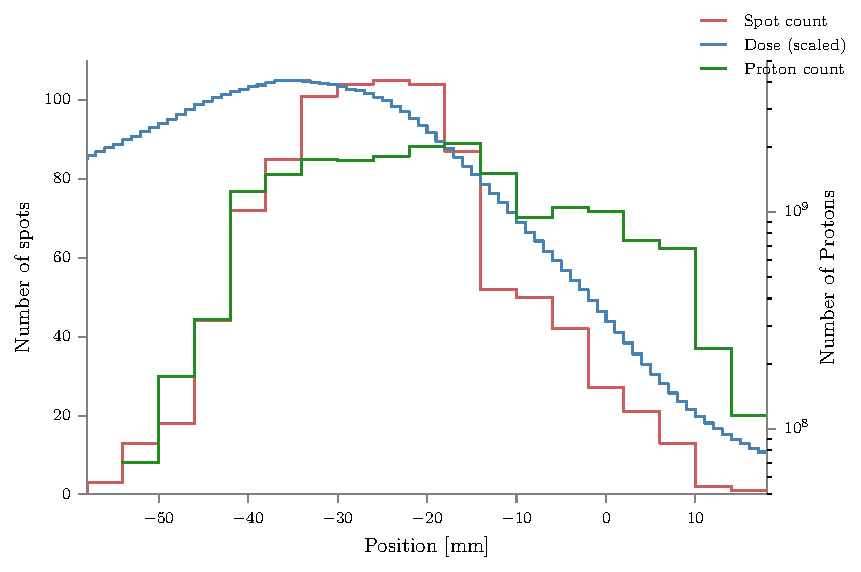
\includegraphics[width=0.99\textwidth]{pics/rtplangeolayers}
\\
}

\headerbox{6. Result Grouping}{name=restwee,below=mettwee,column=2,span=1}{

{\small
\begin{tabular}{lll}
	 & Iso-energy shift & Iso-depth shift\\
	\midrule
	Dose & 6.40 & 6.40 \\
	PG emission & 7.12 & 7.12 \\
	PG + PSF & 4.94 & 6.25 \\
	$\upmu_\Delta$ MPS & 4.72$\pm$1.17 & 5.77$\pm$1.05  \\
	$\upmu_\Delta$ KES & 4.15$\pm$3.82 & 5.15$\pm$2.87  \\
	\midrule
	 & Iso-energy weight & Iso-depth weight \\
	\midrule
	Nr. protons & $1.07\cdot10^9$ & $0.98\cdot10^9$ \\
\end{tabular}
}
}

\headerbox{6. Conclusion}{name=results,below=restwee,column=2,span=1}{
\textbf{Spot-by-spot PG monitoring appears to be unrealistic} given the required statistics for a measurement with millimetric precision and the available statistics in normal and certainly high precision treatment plans. Two spot grouping methods were presented and demonstrated. The precision of the shift improved with respect to iso-energy grouping for the KES camera (1$\upsigma$ = 3.82 and 2.87 mm, iso-energy and iso-depth resp.), but not for the MPS (1$\upsigma$ = 1.17 and 1.05 mm, iso-energy and iso-depth resp.). \textbf{It is shown that grouping spots does not necessarily negatively affect the precision} compared to the artificially increased spots, which means some form of spot grouping can enable clinical use of these PG cameras if the sum of the spot weights is at least $10^9$ proton primaries. \textbf{With all spots or spot groups the MPS camera has a better signal compared to the KES}, thanks to a larger detection efficiency and a lower background level due to time of flight selection.

An extended version of this study will be submitted to \emph{Physics in Medicine and Biology}.
}

\headerbox{References}{name=biblio,column=2,below=results,span=1}{
Pinto et al. (2014) Phys. Med. Biol.\\
Priegnitz et al. (2014) Phys. Med. Biol.\\
Huisman et al. (2016) Phys. Med. Biol.
}

%\headerbox{Acknowledgments}{name=ack,column=2,below=biblio,span=1}{
%This work was partly supported by SIRIC LYric Grant INCa-DGOS-4664, LABEX PRIMES (ANR-11-LABX-0063 / ANR-11-IDEX-0007) and Fondation ARC.
%}

\end{poster}%
\end{document}
